\section{Physics and Algorithms}
\subsection{Physical Equations}
\label{sec.physical.eq}
The spatial and temporal evolution of a compressible fluid is governed by the
Euler equations. The Euler equations are a set of hyperbolic conservation laws
governing the density $\rho$, velocity $\mathbf{v}$, and total specific energy
$E$ (specific kinetic energy $\frac{1}{2}\rho \mathbf{v}^2$ plus specific internal
energy $u$). These quantities $\mathbf{U}$ and their respective fluxes
$\mathbf{F}(\mathbf{U})$, defined through the Euler equations, are conveniently
expressed in vector form as
%
\begin{equation}
    \mathbf{U} =
    \left(
    \begin{array}{c}
        \rho \\
        \mathbf{v} \\
        \rho e \\
    \end{array} \right),
    \quad
    \mathbf{F}(\mathbf{U}) =
    \left(
    \begin{array}{c}
        \rho\mathbf{v} \\
        \rho\mathbf{v}\mathbf{v}^T + P \\
        \rho e\mathbf{v} + P\mathbf{v} \\
    \end{array}
    \right),
\end{equation}
%
where P is the pressure. In this notation the Euler equations can be expressed
in the form
%
\begin{equation}
    \label{eq.euler}
    \frac{\partial \mathbf{U}}{\partial t} + \div \mathbf{F} = 0.
\end{equation}
%
As stated the system of equations are not closed; there are more variables then
equations. Thus, a constraint is needed and is supplied by the equation of state, which is typically given by the ideal gas relation
%
\begin{equation}
    P = \rho(\gamma - 1)u,
\end{equation}
%
where $\gamma$ is the ratio of specific heats.

These equations can be solved by the finite-volume approach, which is a
discretization of the domain into finite sized disjoint cells and evolves their
spatial averaged $\mathbf{U}$ values. Specifically, applying equation
(\ref{eq.euler}) to every cell $i$ with volume $V_i$ and performing Gauss'
theorem to convert the volume integral to a surface integral results in
%
\begin{equation}
    \label{eq.euler.int}
    \frac{d\mathbf{Q}_i}{dt} =
    -\sum_{j}\int\mathbf{F}_{ij}(\mathbf{U})\cdot\mathbf{A}_{ij},
\end{equation}
%
where $\mathbf{A}_{ij}$ is the cell's surface area normal and $\mathbf{Q}_i$
is the volume integral of $\mathbf{U}_i$,
%
\begin{equation}
	\mathbf{Q}_i =
    \left(
    \begin{array}{c}
    	m_i \\
        \mathbf{p}_i \\
        E_i
     \end{array}
     \right) = \int_{V_i}\mathbf{U}_i dV,
\end{equation}
where $m_i$, $\mathbf{p}_i$ and $E_i$ are cell's total mass, momentum, and
energy, respectively. Here, an assumption is taken that the cell's volume
is a polyhedron such that the surface integral can become a sum over all
polygon faces. Additionally, time is discretized leading to a finite difference
update of the cell's quantities given by
%
\begin{equation}
    \label{eq.flux.update}
    \mathbf{Q}_i^{n+1} = \mathbf{Q}_i^n - \Delta t\sum_j
    \mathbf{\hat{F}}_{ij}^{n+1/2} A_{ij}.
\end{equation}
%
In this expression, the flux $\mathbf{\hat{F}}^{n+1/2}$ is taken to be a time
average and is constant across the cell face. To be able to use equation
\ref{eq.flux.update} we must make estimates of
$\mathbf{\hat{F}}^{n+1/2}$ and $A_{ij}$ to the proper order of accuracy. Sections \ref{sec.riemann} and
\ref{sec.tessellation}, respectively, will go into detail on how these quantities are
estimated.

\subsection{Tessellation}
\label{sec.tessellation}
As stated in Section \ref{sec.physical.eq}, the Euler equations, as written in
(\ref{eq.flux.update}), assume that the cells are in the form of polyhedrons.
There are many ways of partitioning space that meet this criteria but for this
paper we will restrict our attention to the Voronoi tessellation. The Voronoi
tessellation partitions the space into a set of disjoint polyhedrons for a
given set of points. The set of points are called mesh generators and for each
generator there is a corresponding region consisting of all points that are closer
to that generator than any other. Thus, for each mesh generating pair there
lies a polygon that is equidistant. This geometric property will be exploited
in several ways. For the rest of this paper we will refer to the polyhedra
associated with the mesh generator as a cell and the polygons making up the
polyhedra as faces.
\begin{figure}
    \begin{center}
        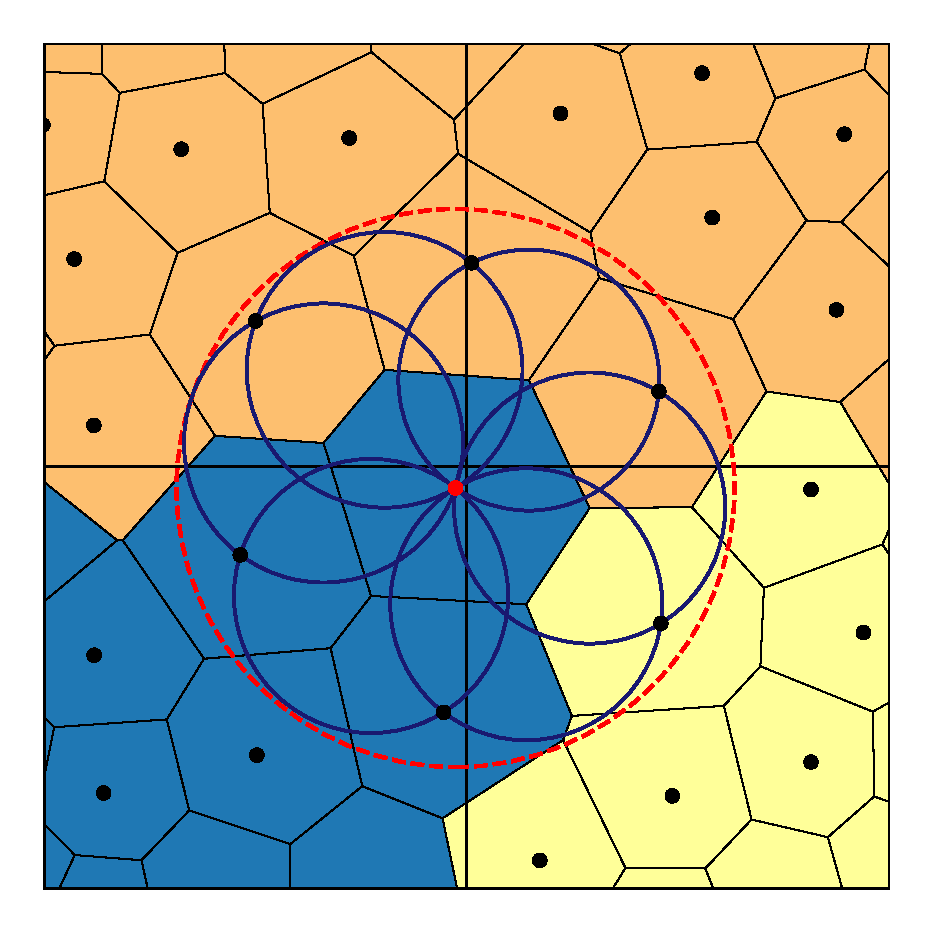
\includegraphics[width=0.5\textwidth]{figures/voronoi.eps}
        \caption{L1 norm of linear wave problem in 2d. Blue points are results}
    \end{center}
\end{figure}

The creation of the Voronoi tessellation can be performed by first constructing
the Delaunay triangulation. The Delaunay tessellation is the dual graph of the
Voronoi tessellation and is defined as the triangulation of points such that
no point in the set lies inside the circumcircle of any of the triangles, in
2d. In 3d the triangles become tetrahedron but the same definition applies.
Remaining in 2d for simplicity, the points are the vertices of the triangles.
The dual aspect refers to the fact that each triangle edge corresponds to a
Voronoi face and each Voronoi vertex corresponds to the center of the
circumcirlce of the triangle. 

\subsection{Fluid Update}
\subsubsection{Reconstruction}
% Need some introductory text
To solve the Riemann problem, primitive values are needed at the face. As a first
choice, cell center values can be used. Although for more accurate results a 
method is needed to extrapolate the cell center values to the center of mass of 
the face. At first order, in space and time, can be constructed by Taylor-series 
expanding the primitive values
%
\begin{equation}
	\label{eq.taylor}
	\mathbf{W}' = \mathbf{W} + \frac{\partial\mathbf{W}}{\partial\mathbf{r}}
    	(\mathbf{f}-\mathbf{s}_i) + \frac{\partial\mathbf{W}}
        {\partial t}{\Delta t}.
\end{equation}
%
The expansion has two unknowns, the spatial derivative
$\frac{\partial\mathbf{W}}{\partial \mathbf{r}}$ and the time derivative
$\frac{\partial\mathbf{W}}{\partial t}$. However, both derivatives
are related through the Euler equations in primitive form
%
\begin{equation}
	\label{eq.time.derivative}
    \frac{\partial\mathbf{W}}{\partial t}  + \mathbf{A}
    	(\mathbf{W})\frac{\partial\mathbf{W}}{\partial\mathbf{r}} = 0,
    \quad
    \mathbf{A}(\mathbf{W}) =
    \left(
    \begin{array}{ccc}
        \mathbf{v} & \rho & 0 \\
        0 & \mathbf{v} & 1/\rho \\
        0 & \gamma P & \mathbf{v}
    \end{array}
    \right).
\end{equation}
%
Thus, only the spatial derivatives need to be calculated. For the
calculation we follow the method presented in (Springel), which is
summarized below. Given a cell $i$ the components of 
$\frac{\partial\mathbf{W}}{\partial \mathbf{r}}$, which are gradients
of the primitive variables, are given by
%
\begin{equation}
	\nabla\phi_i = \frac{1}{V_i}\sum_{j}A_{ij}
    	\left(\left[\phi_i - \phi_j\right]\right) -
        \frac{\phi_i + \phi_j}{2}
        \frac{\mathbf{r}_{ij}}{r_{ij}}.
\end{equation}
%
The sum is over all neighbors $j$ of particle $i$, $\phi_i$ and
$\phi_j$ are the scalar field values at each cell center respectively,
$\mathbf{r}_{ij} = \mathbf{r}_i - \mathbf{r}_j$ is the separation vector
with magnitude $r_{ij} =|\mathbf{r}_{ij}|$. As constructed, the gradients
are second order in space for smooth flows. However, in the presence of
shocks, numerical instabilities may arise and therefore the reconstruction
must be reduced. To deal with this a slope limiter is used. We employ two
limiters. The first one is the method used by AREPO and begins with
the calculation of
%
\begin{equation}
		\psi_{ij} = \left\{
  		\begin{array}{@{}ll@{}}
    		(\phi_i^{max} - \phi_i)/\Delta \phi &
            	\text{for}\ \Delta\phi_{ij} > 0 \\
            (\phi_i^{min} - \phi_i)/\Delta \phi &
            	\text{for}\ \Delta\phi_{ij} < 0 \\
            1 & \text{for}\ \Delta\phi_{ij} = 0,
  		\end{array}\right.
\end{equation}
%
where $\phi_i^{max} =$ max$(\phi_j)$ and $\phi_i^{min} =$ min$(\phi_j)$ are
the maximum/minimum values across all neighbors of $i$ and
$\Delta\phi_{ij} = \nabla \phi_i \cdot (\mathbf{f}_{ij} - \mathbf{s}_i)$. Then 
the minimum of all $\psi_{ij}$s, associated with each primitive field, is found 
producing a single scalar value
%
\begin{equation}
	\alpha_i = min(1, \psi_{ij})
\end{equation}
%
 that is used to limit the gradient
%
\begin{equation}
	\nabla \phi_i' = \alpha_i \nabla \phi_i
\end{equation}

\subsubsection{Riemann Solve}
\label{sec.riemann}
The Riemann problem consist of two constant states separated by an interface.
The solution to this problem is the formation of three waves emanating from the
interface. These waves are associated with the eigenvalues of the Euler equations
and each carry a jump in the characteristic variables. The goal of the Riemann
solver is to estimate these nonlinear waves and construct the fluxes at the
interface. Four purposes, we have elected to use the HLL, HLLC, and Exact Riemann
solvers. 
 
The HLL solver ignores the contact in solving the Riemann problem. In this case
only two waves are considered.

\subsection{Grid Motion}
As currently constructed the method outlined in solving the Euler equations are 
for static meshes only. In our case we allow the mesh to move, meaning the mesh
generators are given some velocity $\mathbf{w}_i$. Thus, equation \ref{eq.euler}
must be augmented to account for an advection term produced by the movement
of the face. The updated Euler equations become
%
\begin{equation}
	\label{eq.euler.moving}
    \mathbf{F}_m(\mathbf{U}) = \mathbf{F}_s(\mathbf{U})
    	- \mathbf{U}\mathbf{w}^T =
    \left(
    \begin{array}{c}
        \rho\mathbf{v} \\
        \rho\mathbf{v}\mathbf{v}^T + P \\
        \rho e\mathbf{v} + P\mathbf{v} \\
    \end{array}
    \right) -
    \left(
    \begin{array}{c}
        \rho\mathbf{w} \\
        \rho\mathbf{v}\mathbf{w}^T \\
        \rho e\mathbf{w} \\
    \end{array}
    \right).
\end{equation}
%
In practice equation  is not used because of its unstable
numerical behavior (Parkmor). The equation can become numerical stable by
solving the fluxes in the rest frame of the face. At the face the conserved 
variables and fluxes become
%
\begin{equation}
	\mathbf{U}' =
    \left(
    \begin{array}{c}
        \rho \\
        \rho(\mathbf{v-w}) \\
        \rho e' \\
    \end{array} \right),
    \quad
   	\mathbf{F}'(\mathbf{U}') = 
    \left(
    \begin{array}{c}
        \rho(\mathbf{v-w}) \\
        \rho(\mathbf{v-w})(\mathbf{v-w})^T + P \\
        \rho e'(\mathbf{v-w}) + P(\mathbf{v-w}) \\
    \end{array}\right) =
    \left(
        \begin{array}{c}
        F_\rho' \\
        F_\mathbf{v}' \\
        F_e' \\
    \end{array}
    \right).
\end{equation}
%
Notice $\rho$ and $P$ remain unchanged however the $e$ transform to
$e' = e -\frac{1}{2}\mathbf{v}^2 + \frac{1}{2}(\mathbf{v-w})^2$. Now
the fluxes need to be transformed back to the lab frame
%
\begin{equation}
	\label{eq.euler.face}
    \mathbf{F}_m(\mathbf{U}) = \mathbf{F}_s(\mathbf{U})
    	- \mathbf{U}\mathbf{w}^T = \mathbf{F}'(\mathbf{U}') +
    \left(
    \begin{array}{c}
        0 \\
        \rho\mathbf{w}(\mathbf{v-w})^T \\
        \rho(\mathbf{vw})(\mathbf{v-w}) -\frac{\rho}{2}
        	\mathbf{w}^2(\mathbf{v-w}) + p\mathbf{w} \\
    \end{array}
    \right),
\end{equation}
%
where the terms have been picked to make equation \ref{eq.euler.face} consistent with
equation \ref{eq.euler.moving}. This equation can be restated in terms of the rest
frame fluxes,
%
\begin{equation}
	\label{eq.final.euler}
    \mathbf{F}_m(\mathbf{U}) = \mathbf{F}_s(\mathbf{U})
    	- \mathbf{U}\mathbf{w}^T = 
    \left(
    \begin{array}{c}
        F_\rho' \\
        F_\mathbf{v}' + \mathbf{w} F_\mathbf{v}'^T \\
        \mathbf{w}F_\mathbf{v}' + \frac{1}{2}F_\rho' \mathbf{w}^2
    \end{array}
    \right).
\end{equation}
%
Thus, after solving the riemann problem in the rest frame of the face the fluxes
can be easily transformed back into the lab frame. Finally, to make use of equation
\ref{eq.final.euler} with \ref{eq.taylor} the primitive variables need to transformed
by the following
%
\begin{equation}
    \mathbf{W}' = \mathbf{W} - 
    \left(
    \begin{array}{c}
        0 \\
        \mathbf{w} \\
        0 \\
    \end{array}
    \right).
\end{equation}
%
This ensures that the correct values are used in the riemann solver.

\subsubsection{Time Integration}
\label{sec.time.integration}
The time integration using equation \ref{eq.euler.int} with \ref{eq.taylor} is
a form of the MUSCL-Hancock scheme. For static meshes, the scheme is second
order accurate in space and time. However, letting the mesh move introduces
inaccuracies due to ignoring the effect of the mesh deformation during a time 
step $\Delta t$. This can be corrected by adopting a Runge-Kutta type scheme, that
uses information from the beginning and the end of a time step instead of mid
point estimations. Specifically, we employ the method outlined by (Pakmor)
which updates the conservative variables by the following
\begin{equation}
	\begin{array}{rcl}
		\mathbf{W}_i' & = & \mathbf{W}_i^n + 
        	\Delta t\frac{\partial\mathbf{W}}{\partial t}, \\
        \mathbf{r}' & = & \mathbf{r}^n + \Delta t\mathbf{w}^n, \\
        \mathbf{Q}_i^{n+1} & = & \mathbf{Q}_i^n -
        	\frac{\Delta t}{2}\left(\sum_j A_{ij}^n\mathbf{\hat{F}}_{ij}^n
            (\mathbf{W}^n) + \sum_j A_{ij}'\mathbf{\hat{F}}_{ij}'
            (\mathbf{W}')\right), \\
        \mathbf{r}^{n+1} & = & \mathbf{r}'.
    \end{array}
\end{equation}
Here we are taking an average of the fluxes from the beginning and the end
of the time step. The flux at the beginning of the time step is constructed
with the current state of the mesh with the primitive values extrapolated to
the face. Then the mesh generators move to their final position
and the mesh is reconstructed. A new flux is constructed with new geometric
quantities, however, the primitive values have been extrapolated in time from
the beginning of the time step. At first glance, it seems that the mesh has
to be constructed twice per time step. However, the generator velocity is
treated constant throughout the time step resulting the final mesh to be equal to
the beginning mesh of the next time step. Thus, the mesh need only to
be constructed once per time step while the fluxes have to be calculated
twice per time step. This method is not truly a Runge-Kutta scheme because
of the time extrapolation but more a mixture of Runge-Kutta and MUSCL-Hancook
scheme that has been shown to be second order accurate in space and time.

\subsubsection{Regularization}
Allowing the mesh generators to move with the local fluid velocity 
$\mathbf{w}_i$ can lead to cells that are elongated or mesh generators close to 
given face. This results, to an unstable evolution of the cells because their 
faces can move rapidly relative to the generator velocity (Duffell). To 
counteract this issue (Springel) proposed a correction term that would steer the 
generator towards its center of mass. This effectively causing the cell to 
become rounder, thus mitigating the issue. The correction term is defined as
%
\begin{equation}
	\mathbf{w}_i' = \mathbf{w}_i + \chi\left\{
  		\begin{array}{@{}ll@{}}
    		0, & \text{for}\ d_i/(\eta R_i) < 0.9 \\
    		c_i\frac{\mathbf{s}_i - \mathbf{r}_i}{d_i}
            	\frac{d_i-0.9\eta R_i}{0.2\eta R_i}, 
            	& \text{for}\ 0.9 \leq d_i/(\eta R_i) < 1.1 \\
            c_i\frac{\mathbf{s}_i - \mathbf{r}_i}{d_i},
               	& \text{for}\ 1.1 \leq (d_i)/(\eta R_i).
  		\end{array}\right.
\end{equation}
%
Here $R_i$ is the effective radius of the cell, $(V_i/\pi)^{1/2}$ for 2d and
$(3V_i/4\pi)^{1/3}$ for 3d, $d_i$ is the distance between the generators
position $\mathbf{r}_i$ and center of mass $\mathbf{s}_i$, $c_i$ is the local sound speed. $\chi$ and $\eta$ are tunning parameters which are typically set 
to 0.25 and 1.0, respectively.

\subsection{External Boundary Conditions}
For each simulation a boundary condition must be defined. At this moment, only
reflection and periodic boundaries are implemented. Our domains are restricted to
rectangular domains with arbitrary aspect ratios. The implementation of both
boundaries make use of ghost particles. These ghost particles are created during
the mesh construction and carry all particle information to participate in the 
integration step. From the simulation perspective, they are treated as real particles,
however, after a time step all ghost particles are discarded and new ghost particles
are formed with the relevant updated particle information.

\subsubsection{Periodic}
Periodic boundaries are formed by examining the circumcirlce of each real particle
in the tessellation. If this value intersects the domain boundary the particle is
flagged for ghost construction. The flagged particle is then shifted periodically in
all dimensions including corner cases and tested for boundary intersection. If 
intersection occurs a ghost particle is formed from the particle but with the
appropriate position data.

\subsubsection{Reflecting}
The reflection boundary parallels the periodic case with exception that particles
are not periodically shifted. Instead, the flagged particle is mirrored across the
minimum and maximum of each boundary dimension. If intersection occurs, again, a ghost
particle is formed, however, the sign of the normal velocity component is flipped.
This ensures that the mass flux vanishes on the surface of the boundary.

\subsection{Gravity}
\label{sec.gravity}
In the presence of gravity the Euler equations \ref{eq.euler} are modified by
a source term
%
\begin{equation}
    \frac{\partial \mathbf{U}}{\partial t} + \div \mathbf{F} =\left( 
    \begin{array}{c}
    	0 \\
        -\rho\nabla\mathbf{\Phi} \\
        -\rho\mathbf{v}\nabla\mathbf{\Phi}
    \end{array}\right).
\end{equation}
%
Note that the gravitational potential $\mathbf{\Phi}$ only affects the
momentum and energy. The source of the potential can be prescribed by
an external source or by the self gravity of the gas. In the latter case
the potential is given by Poisson's equation
%
\begin{equation}
	\label{eq.poisson}
	\nabla^2\mathbf{\Phi} = 4\pi G\rho
\end{equation}
For the moment assume that $\mathbf{\Phi}$ is given. Then the equations
\ref{eq.taylor} and \ref{eq.euler.int} can be easily supplemented to
include the gravitational force. First, the time derivatives in the
reconstruction equation are replaced by
%
\begin{equation}
	\label{eq.primitive.gravity}
    \frac{\partial\mathbf{W}}{\partial t}  + \mathbf{A}
    	\left(\mathbf{W}\right)\frac{\partial\mathbf{W}}{\partial\mathbf{r}}
        = \left(
        	\begin{array}{c}
            0 \\
            -\nabla\mathbf{\Phi} \\
            0
            \end{array}
         \right),
\end{equation}
%
In this case the time extrapolated variables include a gravitational
component. Second, the momentum and energy is updated during the flux update
%
\begin{equation}
	\label{eq.gravity.update}
	\begin{array}{rcl}
        \Delta\mathbf{p}_i & = &
        	\frac{\Delta t}{2}\left(\sum_j A_{ij}^n\mathbf{\hat{F}}_{ij,\mathbf{p}}^n
            (\mathbf{W}^n) + \sum_j A_{ij}'\mathbf{\hat{F}}_{ij,\mathbf{p}}'
            (\mathbf{W}')\right) - \frac{1}{2}\Delta t\left( 
        	m_i\nabla_i\mathbf{\Phi} + m_i'\nabla_i\mathbf{\Phi}'\right)\\
        \Delta E_i & = &
        	\frac{\Delta t}{2}\left(\sum_j A_{ij}^n\mathbf{\hat{F}}_{ij,E}^n
            (\mathbf{W}^n) + \sum_j A_{ij}'\mathbf{\hat{F}}_{ij,E}'
            (\mathbf{W}')\right) - \frac{1}{2}\Delta t\left( 
        	m_i\mathbf{v}_i\nabla_i\mathbf{\Phi} +
            m_i'\mathbf{v}_i'\nabla_i\mathbf{\Phi}'\right).\\
    \end{array}
\end{equation}
%
\subsubsection{Constant}
In the simplest case, the gravitational field can be defined as a constant external field. This assumes
that the self gravity component of the gravitational field is negligible compared to the external field.
In this case $\rho$ can be set to zero and the solution to Equation~\ref{eq.poisson} becomes trivial
\begin{equation}
	-\nabla\mathbf{\Phi} = \mathbf{g},
\end{equation}
where $\mathbf{g}$ is a constant field. Once $\mathbf{g}$ is specified it can be coupled with the fluid
equations through Equations \ref{eq.primitive.gravity} and \ref{eq.gravity.update}.

\subsubsection{Tree}
In the general case self gravity should be taken into account. Because 
gravity is a long range force and the typical high density range
seen in astrophysical problems, the calculation of the gravitational forces
can be particularly challenging. The root of the problem
is the $N-1$ calculation per particle in the direct sum approach. Calculating the force for
each particle, produces a solver that scales as $\mathcal{O}(N^2)$ which is intractable.
The scaling problem can be remedy by a Tree based solver (\cite{Barnes1986}; hereafter BH).
In this scenario the particles
are broken into a hierarchy of groups, with their own multipole value, dictated by a 
recursive spatial subdivision scheme. The hierarchy, combined with a suitable
criteria to transverse it, can be used to approximate the force calculation in
$\log{}N$ operations per particle. Thus the $\mathcal{O}(N^2)$ scaling produced by the direct sum
approach can be approximated by an operation that scales as $\mathcal{O}(N\log{}N)$.

The first part in constructing a Tree based solver is picking a grouping scheme.
Our spatial decomposition scheme is based on the BH algorithm. In this scheme
the domain is placed inside a cubic node, called the root. The root contains 8 daughter nodes in
3D (4 daughter nodes in 2D) that
subdivides the space evenly. Particles are added to the root in a one by one basis. For each particle
the root searches for the daughter node that spatially contains the particle. Once found, the daughter
node will have three possible scenarios. First, if the node does not have any daughter nodes and does
not store a particle then the particle is placed there and the node is termed a ``leaf'' node.
Second, if the node already has a daughter node then the search continues recursively. Third,
if the node already has a particle stored then the node is recursively subdivided until
both particles exist in their own respective leaf nodes. Once all the particles are processed
the multipole for each node can be calculated recursively.

With the Tree constructed the force for a given particle can be approximated by ``walking'' the
Tree. This procedure is performed by starting at the root. Using a specified criteria a decision
is made if including the nodes multipole provides an accurate force calculation. If it does
then the multipole value is used and the walk along this branch is terminated. If the multipole 
is not suitable then the node is ``opened'' and the procedure is repeated for each daughter node.
The BH criteria to open a node is
\begin{equation}
\frac{l}{r} \ge \alpha,
\end{equation}
where $l$ is the side length of the node, $r$ is the distance between the particle and the center mass
of the node, and $\alpha$ is a free parameter constrained to $0 \le \alpha \le 1$. The error is 
effectively controlled by $\alpha$ because decreasing $\alpha$ produces walks with increasing lower
level nodes. At the extreme case, setting $\alpha=0$ opens every node and the computation becomes
the original direct sum approach.

At this point, our description of the Tree solver has been purely a serial implementation. In a parallel
simulation the algorithm has to be slightly modified. We follow the approach of \cite{Springel2005}. In
this approach each processor build its local BH Tree. Moreover, the local tree is augmented with
``pseudo-particles'' that serve as place holders for branches from different processors. Once the local
multipole values are computed locally they are communicated across all processors. In doing so, each
local tree can now construct the global ``top-tree''. The local Tree is consistent in the sense that all
internal nodes have the correct multipole. Now that the Tree is consistent a Tree walk can be performed.
However, if particle opens a pseudo-particle it is flagged for export and placed in a communication
buffer. Once the buffers are full the particles are exchanged and remote walks are performed. The
particles are finally returned to their local processor with correct force calculation.

\subsection{Parallelism}
\label{sec.parallel}
\subsubsection{Partitioning}
For domain decomposition we use a Hilbert-Peano space filling curve \citep{Springel2005}. A space
filling curve maps 3D positions onto a 1D curve. A Hilbert-Peano curve has the additional property
that it preserves locality. Meaning that points that are close along the 1D curve or generally close
in 3D space. To perform a load balance, the idea is generate a Hilbert key for each particle in
the simulation. Then the keys are sorted and partitioned with roughly equal work across the processors.

\begin{figure}
    \begin{center}
        \includegraphics[width=0.9\textwidth]{figures/load-balance.eps}
        \caption{L1 norm of linear wave problem in 2d. Blue points are results}
    \end{center}
\end{figure}

In practice, each dimension of the particle is mapped to the integer interval
of $[0, 2^n-1]$, where n is the number of bits per dimension. The parameter
$n$ may be thought as resolution level of the domain similar to AMR codes. For example,
when $n=1$ the domain is portioned into $2^1\times2^1=4$ cells in 2D. Likewise, if $n=4$
the domain is partitioned into $2^4\times2^4=256$ cells. Therefore every $n$ corresponds
to a level of refinement. Moreover, the total number of cells corresponds to the total
possible number of Hilbert-Peano keys. We typically use values of $n\le 20$ such that
the key fits in 64-bit integer. After the keys are computed for each particle the keys
need to be sorted. However performing a global sort is not a trivial operation. Instead
the keys are sorted locally and partitioned into small segments. Then the segments are shared
across all the processors and segments are further refined by joing and splitting overlaps.
The final result is a series of segments that have roughly constant work load are assigned
to each processor. Geometrically, the segments create a tiling of the space, see figure.
Here we have performed the Sedov simulation see test on 8 processors. On the left hand side
we plot the tiling produce by the segments with particle overlayed color coded by their
residing processor. Further we have plotted the the Hilbert-Peano keys (red line) at $n=4$.
Clearly we can see the segment cuts that produce compact spaces of particles. On the right
hand side we show the Voronoi mesh produced by this decomposition.

\subsubsection{Ghost particle copying}
For ghost particle we make a further distinction, interior and exterior ghost particles.
Interior ghost particles are only used in parallel simulations while exterior ghost
particles are associated with the boundary conditions of the simulation. In the following
section we will go into the details on how the DomainManager creates ghost particles
and transfers data.
